\documentclass[a4paper]{article}
\usepackage{array}  
\usepackage[table]{xcolor}% http://ctan.org/pkg/xcolor
\usepackage{geometry}
\geometry{margin=1.25in}
\usepackage{hhline}
\usepackage{environ}
\usepackage{graphicx}
 %\geometry{
 %a4paper,z
 %total={170mm,257mm},
 %left=40mm,
 %right=40mm
 %}
 \newcommand{\colWidth}{141mm}

\begin{document} 
\section*{Demo day: \textit{(demo   \  \  \  )} Group \textit{(group 10)}}

% ------------GOALS----------

\begin{center}
\begin{tabular}{|p{\colWidth}|}
	\hline
	\cellcolor{blue!25}\large
	\textbf{What were your goals?}
	\\ \hline
	\vtop to 70mm{
\begin{itemize}
    \item B.O.B constructed such that he can move.
    \item B.O.B will be able to move by following a line.
    \item Server Prototype: 
    \begin{itemize}
        \item Get and insert data.
        \item Select route.
    \end{itemize}
    \item App Prototype:
    \begin{itemize}
        \item zeroconf bypass.
        \item Authentication.
        \item View order.
    \end{itemize}
    \item Website Prototype: 
    \begin{itemize}
        \item User authentication.
        \item On and off switch for B.O.B.
    \end{itemize}
\end{itemize}
  }
  \\
  %have database - connects - get order and stuff - FOR SERVER
  \hline
\end{tabular}
\vskip 5mm

% ------------ORGANISATION----------

\begin{tabular}{|p{\colWidth}|}
	\hline
	\cellcolor{blue!25}\large
	\textbf{Summarise how your group organised the workload to achieve your goals.}
	\\ \hline
	\vtop to 75mm{
	\begin{itemize}
	    \item Team Split
	    \begin{itemize}
	        \item Robot Hardware
	        \item Robot Software
	        \item Server, Website and App 
	    \end{itemize}
	    \item Robot Hardware
	    \begin{itemize}
	        \item Jacob modelled B.O.B
	        \item Claire, Alex, and Anna, supported Jacob.
	    \end{itemize}
	    \item Robot Software
	    \begin{itemize}
	        \item Claire, Alex, Anna, and Kieran, implemented B.O.B's motion.
	    \end{itemize}
	    \item Server, Website and App 
	    \begin{itemize}
	        \item Freddie, Oktay and Zach implemented the server.
	        \item Oktay and Freddie implemented the App.
	        \item Harry and Oktay implemented the website.
	    \end{itemize}
	\end{itemize}
  }
  \\
  \hline
\end{tabular}
\vskip 5mm

% ------------ACHIEVEMENTS----------

\begin{tabular}{|p{\colWidth}|}
	\hline
	\cellcolor{blue!25}\large
	\textbf{What were your main achievements?}
	\\ \hline
	\vtop to 25mm{
	\begin{itemize}
	    \item B.O.B follows a line. 
	    \item B.O.B detects markers.
	    \item B.O.B software, website and app connects to server.
	    \item Quick problem-solving when dropping Google FireBase.
	\end{itemize}
  }
  \\
  \hline
\end{tabular}
\vskip 5mm

% ------------NOT ACHIEVED----------

\begin{tabular}{|p{\colWidth}|}
	\hline
	\cellcolor{blue!25}\large
	\textbf{What did you not achieve? Briefly explain why.}
	\\ \hline
	\vtop to 25mm{
	\begin{itemize}
	    \item Using Google Firebase for server implementation due of Wifi restrictions (no internet). Resorted to server implementation being handled locally. 
	    \item Using infrared sensors with Raspberry Pi to follow a line. Resorted to using colour sensors with EV3 for more precision.
	\end{itemize}
  }
  \\
  \hline
\end{tabular}
\vskip 5mm

% ------------NEXT STEPS----------

\begin{tabular}{|p{\colWidth}|}
	\hline
	\cellcolor{blue!25}\large
	\textbf{Say briefly what changes you will make to your plan for the next demo.}
	\\ \hline
	\vtop to 30mm{
	\begin{itemize}
	    \item Reverse motion.
	    \item Offload computation to Raspberry Pi with TCP connection.
	    \item Spreading out more of group members when tackling tasks.
	    \item Construct and test grabbing mechanism.
	    \item Develop app and website further.
	\end{itemize}
  }
  \\
  \hline
\end{tabular}

% ------------QUANTITIVE----------
\newpage
\begin{tabular}{|p{\colWidth}|}
	\hline
	\cellcolor{blue!25}\large
	\textbf{Include any quantitative data you have collected (this can be a graph/table with a few words)}
  \\
  \hline
\end{tabular}
\begin{figure}[!htb]
\minipage{0.45\textwidth}
  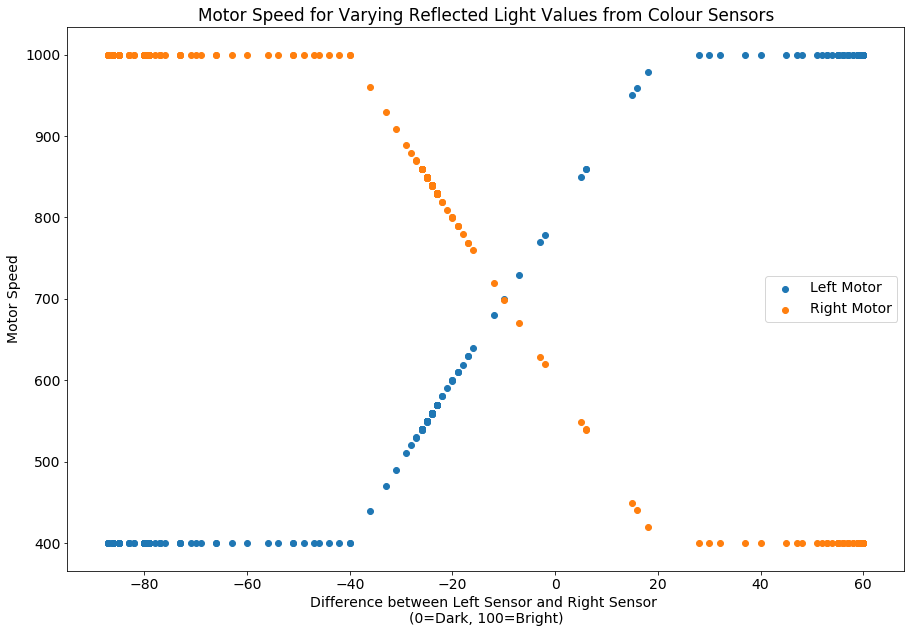
\includegraphics[width=\linewidth]{motor_colour.png}
  \caption{Difference of sensor readings with regards to motor speed.}\label{fig:awesome_image1}
\endminipage\hfill
    \minipage{0.55\textwidth}
     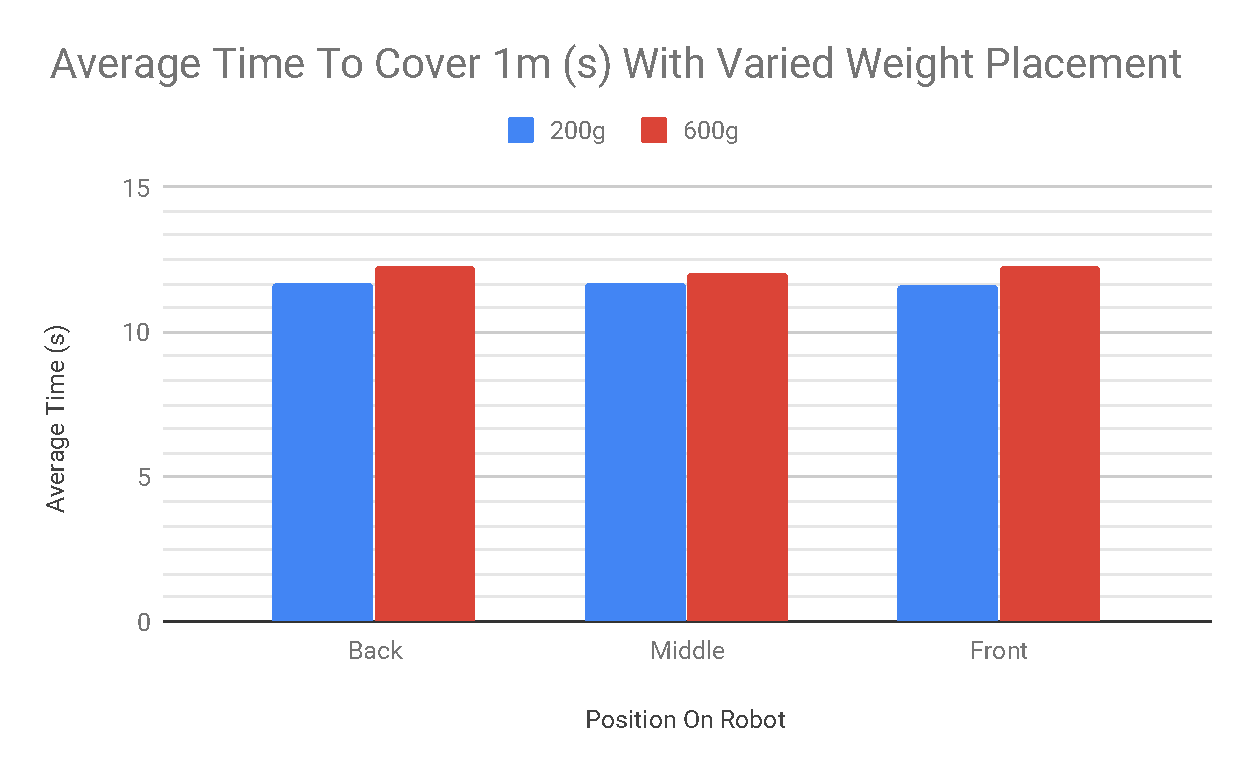
\includegraphics[width=\textwidth]{time_weight.pdf}
     \caption{Affect of varied weights when covering 1 meter}\label{fig:awesome_image2}
\endminipage\hfill
\minipage{0.50\textwidth}
      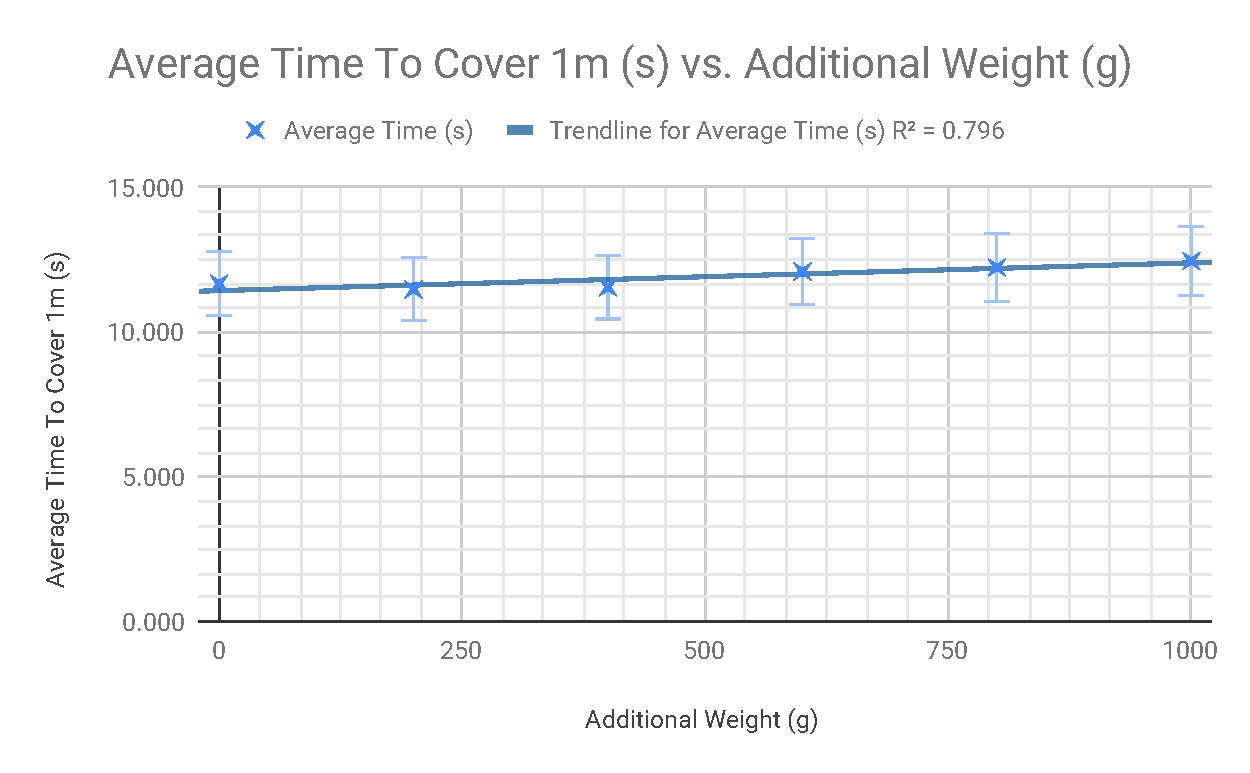
\includegraphics[width=\textwidth]{time_weight2.pdf}
      \caption{Impact of additional weights when covering 1 meter}\label{fig:awesome_image3}
\endminipage
\minipage{0.50\textwidth}
      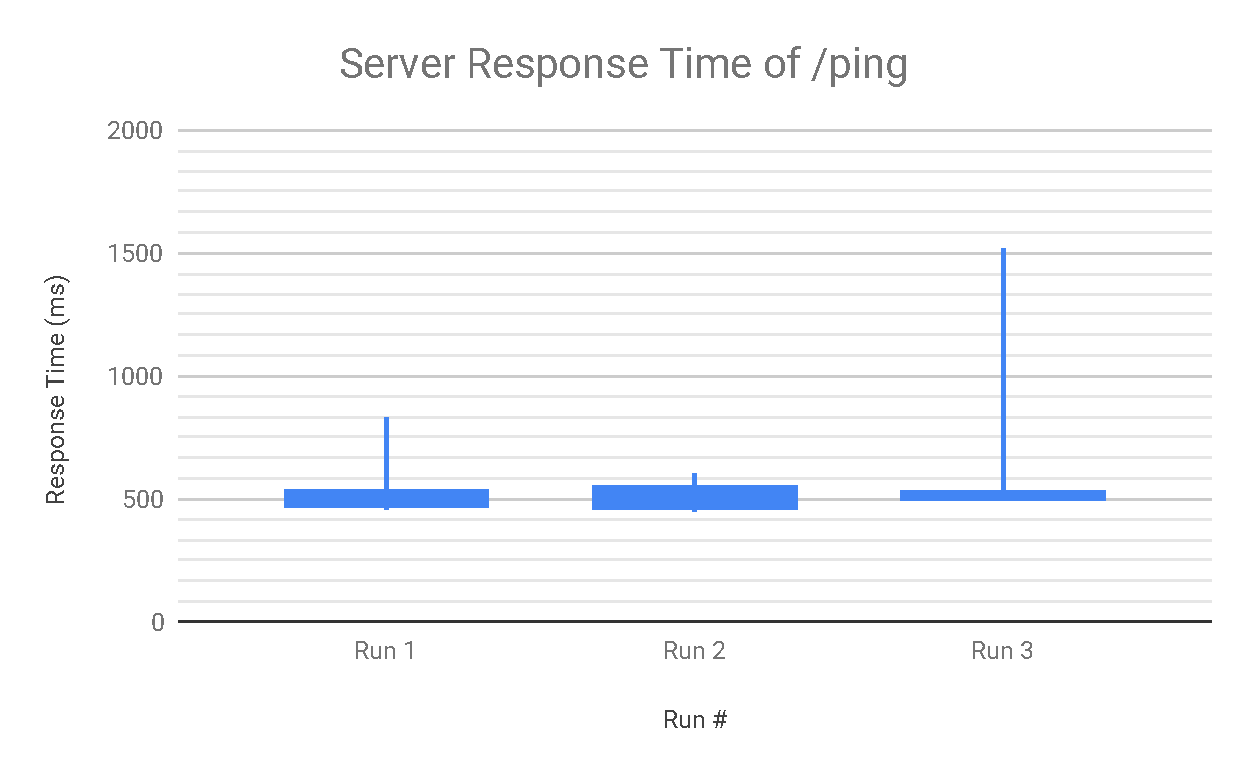
\includegraphics[width=\textwidth]{time_ping.pdf}
      \caption{Server response time when pinging}\label{fig:awesome_image4}
\endminipage
\newline
\end{figure}
\begin{table}[!htb]
\centering
\begin{tabular}{| p{2cm} | p{2cm} |}
\hline
\textbf{Battery (mAh)} & \textbf{Voltage} \\
\hline
2200 & 7.5V \\
\hline
\end{tabular}
\caption{EV3 Battery and Voltage}
\end{table}
\begin{table}[!htb]
\centering
\begin{tabular}{| p{2.2cm} | p{2cm} | p{2.2cm} | p{2cm} | p{2cm} |}
\hline
\textbf{Component} & \textbf{Amperes (7.5V)} & \textbf{Number on Board} & \textbf{Total Amperes} & \textbf{Total mA}\\
\hline
Colour Sensor & 0.107 & 3 & 0.321 & 321 \\
\hline
Motor (Running at 100\%) & 0.186 & 3 & 0.558 & 558 \\
\hline 
Processor (Running at 100\%) & 0.098 & 1 & 0.098 & 98 \\
\hline
\textbf{Battery Time From Full Charge (Hours)} & & & & 2.52 \\ 
 \hline
\end{tabular}
\caption{Source https://www.dexterindustries.com/ev3-current-consumption-measurement/}
\end{table}
\end{center}
  
\end{document}
